\newpage
\textbf{\textcolor{MidnightBlue}{2.}}
Considera la ejecución de la figura 1. Haz lo siguiente:
\begin{enumerate}[a)]
%%%%%%%%%%%%%%%%%%%%%%%%%%%%        Inciso A        %%%%%%%%%%%%%%%%%%%%%%%%%%%%%%%%%%
\item Ejecuta el algoritmo de relojes lógicos y asigna el tiempo lógico a cada evento.
%%%%%%%%%%%%%%%%%%%%%%%%%%%%        Inciso B        %%%%%%%%%%%%%%%%%%%%%%%%%%%%%%%%%%
\item Ejecuta el algoritmo de relojes vectoriales y asigna el vector de tiempo
a cada evento.
%%%%%%%%%%%%%%%%%%%%%%%%%%%%        Inciso C        %%%%%%%%%%%%%%%%%%%%%%%%%%%%%%%%%%
\item Muestra dos cortes consistentes y dos inconsistentes.
\end{enumerate}
\begin{center}
    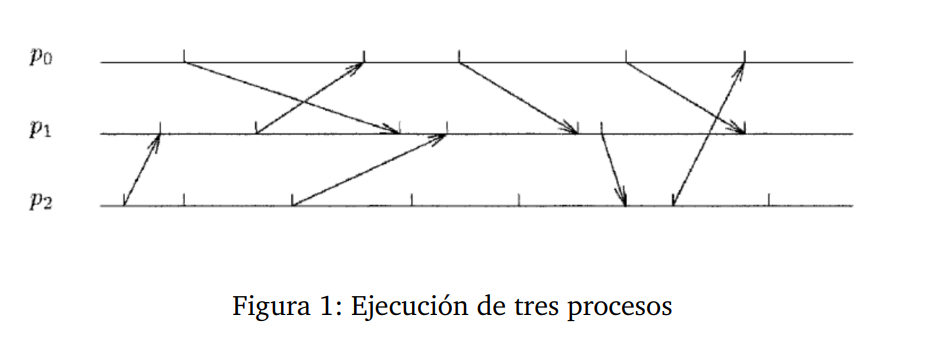
\includegraphics[scale=0.5]{Grapho.png}
    \end{center}
